\chapter{Results}

In this chapter, we present the results of the method explained previously.

\begin{enumerate}
    \item Sensor Space: We start by studying the data in the time-frequency space to find the most important times and frequencies ranges:
          \begin{enumerate}
              \item The classification by CSP allowed us to obtain a time-frequency map, which allows associating to each time and frequency a roc-auc. This roc-auc indicates to what extent the information stored in the working memory is decodable by geometric information.
              \item The permutation statistics allow to extract the most informative time-frequency cluster, as well as to check the significance of the results.
          \end{enumerate}

    \item Source space: After having verified the statistical significance of our cluster, we use this cluster to project the information in a three-dimensional space, (aka the source space), in order to visualize the contrast between the working memory loaded with 3-items versus 1-item. It is mainly this step that allows us to extract the neuroanatomical information.
\end{enumerate}

\section{Sensor space results}

\subsection{CSP results}


\begin{figure}
    \centering
    \begin{subfigure}{.5\textwidth}
        \centering
        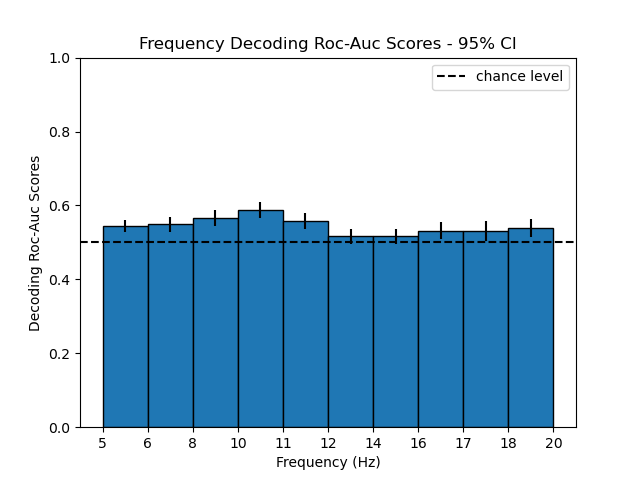
\includegraphics[width=1.\linewidth]{images_report/sensor/csp_permutation_res/csp_frequency.png}
        \caption{CSP frequency decoding.}
        \label{fig:csp_frequency}
    \end{subfigure}%
    \begin{subfigure}{.5\textwidth}
        \centering
        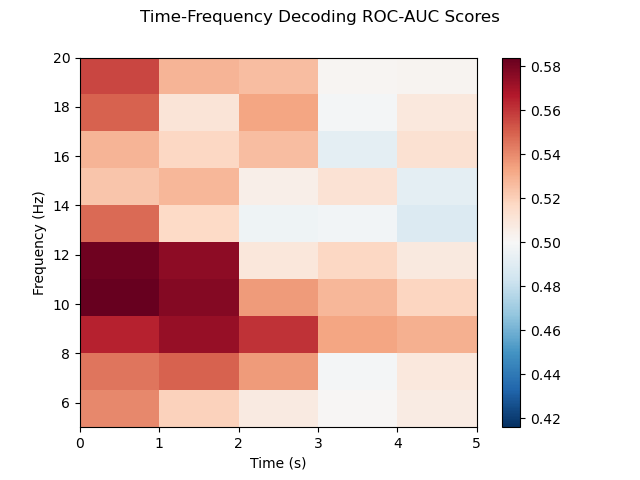
\includegraphics[width=1.\linewidth]{images_report/sensor/csp_permutation_res/csp_time_frequency.png}
        \caption{CSP time-frequency decoding.}
        \label{fig:csp_time_frequency}
    \end{subfigure}
    \caption{CSP results for the average subject.}
    \label{fig:csp_results}
\end{figure}


% [expliquer avant que le CSP est appliqué pour différentes bins et que l'on compare par la suite le roc auc score pour différentess bins, ce qui permet de mettre les régions d'interet en ]

In the figure \ref{fig:csp_results}, we observe the roc-auc score of the classifier composed of (CSP, logistic regression) for different :

\begin{itemize}
    \item frequency ranges distributed linearly between 5 Hz and 20 Hz as well.
    \item time ranges in the reproduction interval, i.e., between $t=0$ and $t=5$ seconds (the figures \ref{fig:Evoked_data}, \ref{fig:decoding_initial} presented the times $t \leq 0$ only for pedagogical purposes).
\end{itemize}

We can see that the CSP algorithm succeeded in highlighting the alpha frequency band between 8 and 12 Hz, and the results are consistent between the frequency map \ref{fig:csp_frequency} and the time-frequency map \ref{fig:csp_time_frequency}, with both a maximal score around 10 Hz.

\subsection{Cluster Permutation Test results}

\begin{figure}[ht]
    \centering
    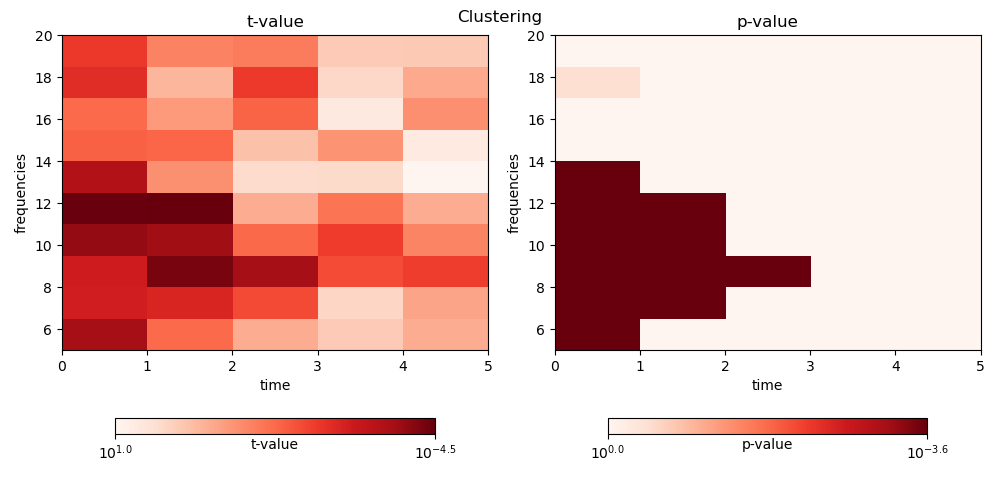
\includegraphics[width=15cm]{images_report/sensor/csp_permutation_res/permutations_test.png}
    \caption[Permutation statistics results.]%
    {Permutation statistics results.}
    \label{permutation_statistics_results}
\end{figure}

The figure \ref{permutation_statistics_results} presents the results of the permutation test cluster. We obtain two clusters of p-values, in low alpha frequency (6 Hz to 14 Hz) and beta (17 Hz-18.5 Hz), of p-values $10^{-3.6}$ and $0.12$ respectively. These clusters indicate that it is necessary to filter on the alpha band at the beginning of the reproduction phase in order to maximize the signal-to-noise ratio when studying the contrast in source space.

\section{Sensor results discussion}

\paragraph{Quantitative analysis}
An AUC of 0.6 is not high in absolute terms, but not bad in EEG analysis on intervals of only 0.5 seconds. If we combine all the bins by bagging, we would get a much better AUC. Furthermore, statistics by clusters permutation show that the results are very significant at the group level.

\paragraph{Qualitative analysis}

Our main cluster is centered on the alpha band. We will discuss the alpha band in more detail in section \ref{section:alpha_discussion}. But we already know from the literature that the alpha band is key to the working memory loads \cite{obleser2012adverse}, which is encouraging.

A surprising phenomenon is that the algorithm can decode much more easily at the beginning of the restitution phase than at the end of the restitution phase. Given that the CSP encodes geometric information, this means that:
\begin{itemize}
    \item either the information in the working memory is transformed in the course of restitution into information disseminated in the brain in a non-geometrical way.
    \item Or, given the very large number of repetitions of the experiment, the subject gets tired after a while and forgets the sequence "instantly" after having repeated it in order to save mental energy.
\end{itemize}



\section{Source space results}


\begin{figure}[ht]
    \centering
    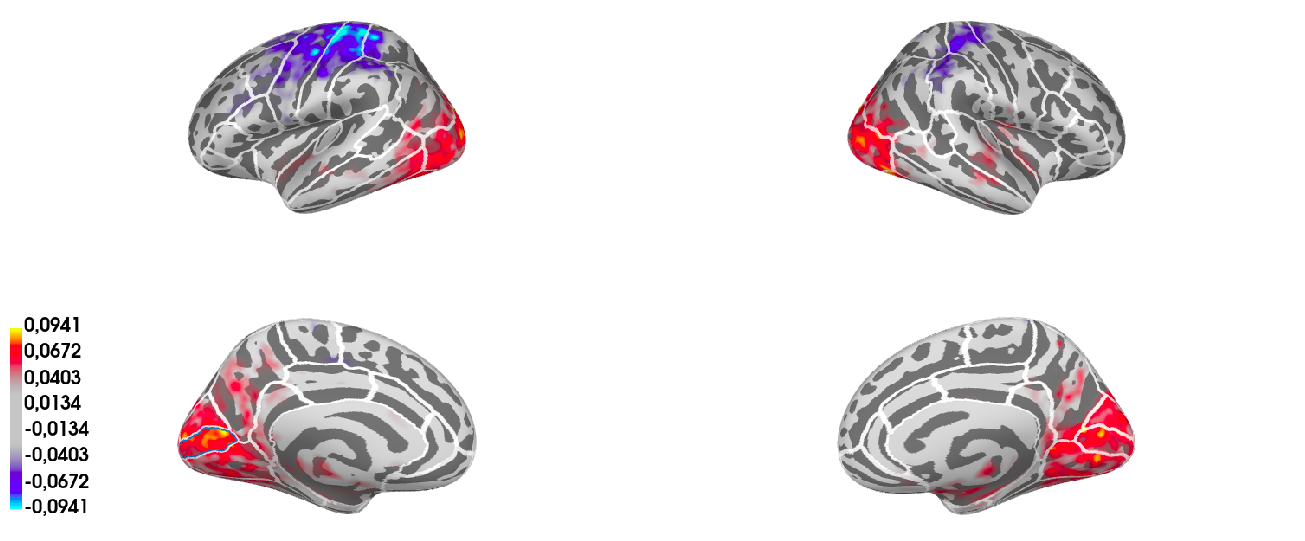
\includegraphics[width=15cm]{images_report/source/source_results_3d_cropped.png}
    \caption[Contrast results in the source space (alpha)]%
    {Contrast results in source space for 0s-1s, and 8Hz-14Hz (alpha).}
    \label{results_source_space_alpha}
\end{figure}

\begin{figure}[ht]
    \centering
    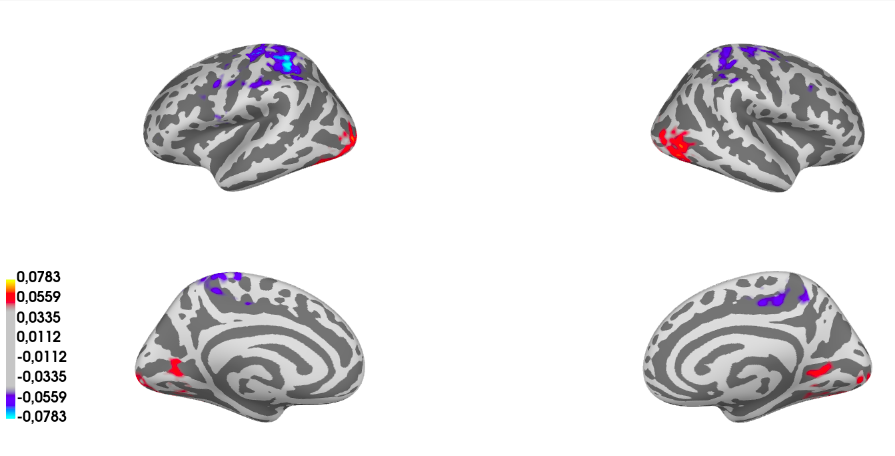
\includegraphics[width=13cm]{images_report/source/source_results_beta_1s.png}
    \caption[Contrast results in the source space (beta)]%
    {Contrast results in source space for 0s-1s, and 15Hz-20Hz (beta).}
    \label{results_source_space_beta}
\end{figure}

The figure \ref{results_source_space_alpha} presents the results of the contrast in source space for the most significant time-frequency bin at the group level, i.e., 0s-1s, and 8Hz-14Hz. In this figure, the red regions are the regions activated for 3 items, while the blue regions are more activated for 1 item. We recall that 3 items are supposed to load the working memory, more than 1 item.

\paragraph{Occipital cortex (visual)}
\label{section:alpha_discussion}
The red region activated here belongs to the visual area. The fact that we see the visual area here is not surprising: we have to remember that we are visualizing here the alpha band, which is a classically inhibitory band in the literature. Thus, the classical interpretation of an activation in the alpha band corresponds to an inhibition of the function of the associated region. This is confirmed by the fact that when we look at the activation in the beta \ref{results_source_space_beta} of our contrast, the activation of the visual cortex (the red region) disappears almost completely.

An increase in the alpha band was an expected classical effect: the literature presents other results similar to this one. For example, \cite{obleser2012adverse} shows that "Enhanced alpha oscillations (8-13 Hz) during retention of items in working memory are often interpreted to reflect increased demands on storage and inhibition".

% Cela montre qu'il y a des similarités entre le stockage de durée et le stockage de contenu discret.

\paragraph{Sensorimotor Areas}

\begin{figure}[ht]
    \centering
    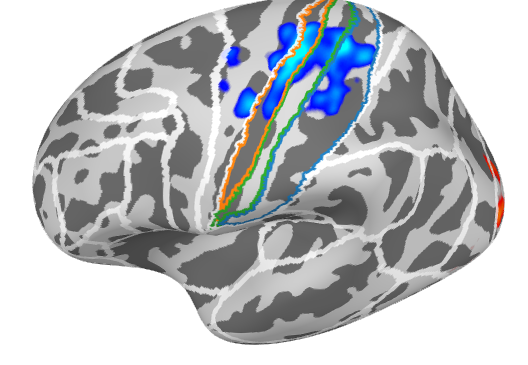
\includegraphics[width=7cm]{images_report/source/brodmann_alpha.png}
    \caption[Focus on the Brodmann areas]%
    {Focus on the Brodmann areas 1 (green), 2 (blue) and 3 (orange), from the alpha band in the left hemisphere.}
    \label{brodmann_alpha}
\end{figure}

The blue region activated at the top of the brain is the sensorimotor area, centered on the postcentral gyrus (Brodmann areas 1, 2 and 3). Before the MEG experiment, subjects were trained to reproduce the task by pressing a button, which explains the activation here. And the region of the somatosensory cortex activated here corresponds to the location of the hand receptors \ref{brodmann_alpha}. This is also supported by the fact that the activation is stronger in the left hemisphere, which is consistent with the fact that the subjects are right-handed.

A possible interpretation is that time is represented by the preparation of the movement of one of the body parts, here the hand. We can also reason by analogy by noting that musical children learn to master rhythms by beating the beat or walking to the rhythm of the pulse. The rhythmic information is embodied. Therefore, even if here the analogy has limits since the temporal signal is not organized in a rhythmic and regular way, this interpretation seems to us to be the most natural one.

% La traduction de la commande moteur est sans doute plus directe avec un seul item qu'avec 3 items, mais des analyses complémentaires peuvent être 

\paragraph{Auditory area}

There is no evidence of activation in the visual regions while the cue is an auditory one. There are several interpretations:
— To see an activation in the auditory zones one must place oneself at $t \leq 0$, as on the figures \ref{auditory_cortex}. But here, during the reproduction phase ($t \geq 0$), the auditory cortex is no longer involved.
— The signal is abstracted from the auditory region to transform it into a purely rhythmic information, thus no longer restricted to the auditory areas.
— The auditory region is activated, but we do not see it in this group figure. As a matter of fact, the auditory regions are visible in the CSP components of the subjects as in the figure \ref{fig:csp_component_beta_band}. But there is a lot of inter-subject variability: After looking at the CSP components for the different subjects, it appears that only subjects with a marked beta peak show activation in auditory cortex, and this peak is not restricted to $0 \leq t \leq 1$ but are spread across all subjects between $0s - 5s$. In order to see an auditory signal at the group level, one would have to align and average the first extracted components for each peak from each subject. But averaging the components presents mathematical difficulties (see in annex \ref{section:csp_average_difficulty}), and could be a research topic in itself.

% [Image beta et pour CSP aussi.]\label{section:csp_average_difficulty}

% \section{Discussion}

% encore un résumé